\subsection{Formato}
El punto clave para que el usuario entienda lo que queremos transmitirle es crear una comunicacion fluida entre la representacion
de los datos el usuario. Para ello  deberemos asegurarnos que hablamos el mismo idioma, con un vocabulario facil de entender y
con proximidad, es decir,dejar la terminologia a un lado y comunicar el objetivo de la manera mas simple posible.
Por ello la representacion de la informacion jugaran un papel fundamental para que la 
informacion sea absorbida por el usuario de una manera natural.

\textcolor{red}{\textbf{Por Aqui voy}}

El apartado anterior "Interpretabilidad", vimo que un conjunto de datos en crudo no siempre era el mas adecuado para la mayoria de los usuarios.
Deberemos estudiar que tipo de representacion es mas adecuada, no siempre una grafica es la representacion mas adecuada, deberemos hacer un 
estudio de tanto al publico al que va dirigido como como podemos acentuar la informacion que sea mas relevante en la manera 
correcta.
Si nos declinamos por realizar una representacion con graficas, deberemos estudiar los datos para saber que tipo de grafica. Por ejemplo, si hablamos de muestras y queremos saber la 
densidad, nos inclinaremos por un grafico de densidad y si por ejemplo buscamos la diferencia entre sexos, utilizaremos un grafico de tartas.



\subsubsection{How to solve it} 
Este modelo debera proporcional la informacion al usario en un lenguaje o formato compresible. Si no es posible proporcionarmos las herramientas necesarias para que este pueda 
comprender el contexto de la informacion.
Es importante que proporcionemos la informacion en un idioma que el usuario entienda, ya sea este literal o visual.
Hablamos de vocabulario y terminologia, deberemos huir de los tecnicismo que sumerjan al usuario en una nube de 
imcomprensibilidad, ya que

\subsubsection{How we solve it. Aire Guru} 
Nuestra herramienta utiliza como componenete principal un mapa sobre el que se representa el AQI general calculado. Este es un formato 
mas legible para los usuarios. Este indice mustra un indicador con cinco niveles: "Insalubre" "Malo" "Pobre" "Aceptable" y "Bueno" y 
especifica un rango de colores desde el rojo hasta el celeste.\\
Nuestra plataforma introduce ademas una iconografica para ayudar al usuario a tener una idea directa de la situacion, ya que son mas 
explicativos que los colores. En caso de peligro, queda bien representado con el color rojo, pero en el caso del azul o verde, en nuestra cultura, no
tenemos definido un estado para estos colores.\\
\begin{figure}[ht]
    \centering
    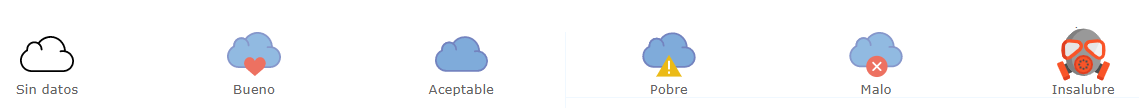
\includegraphics[width=12cm]{EAQUI_Icons}
    \caption{Iconografica Aire Guru}
\end{figure}

Ademas proporciona un glosario con las descripciones de los agentes contaminantes, complicaciones medicas, fuentes de contaminacion
y la iconografia utilizada y una ayuda donde se puede consultar el calculo de AQI y ampliar informacion.

La herramienta Aire guru presenta la informacion en el idioma nativo de la ciudad y se utiliza un lenguaje sencillo y directo.
Ademas se utiliza el mismo estilo, colores e iconografia en todo el diseno para que el usuario se familierize rapidamente y pueda
prestar atencion al significado de los datos en vez de perderse en el diseno e intentar encontrar su significado.
 
\elsparagraph{Evaluation}  
\begin{itemize}
    \done El lenguaje utilizado en toda la herramienta es un lenguaje comun, huye de la terminologia cientifica pero proporciona la informacion
    suficiente para enteder la situacion.
    \crossed Algunos terminos especificos no se han podido sustituir como "Indice de calidad del Aire".
    \done Se han proporcionado la herramientas necesarias para entender el concepto. Se ha utilizado la norma europea de calidad del aire para 
    representar los valores y se ofrece al usuario recursos en la pagina para su comprension ademas de recursos extenos.
    
\end{itemize}
 

\newpage